\documentclass[11pt,oneside]{book}
\usepackage{enumitem}
\usepackage{fancyhdr}
\usepackage[a4paper,top=2cm,bottom=3cm,left=2cm,right=2cm,marginparwidth=1.75cm]{geometry}
\usepackage{hyperref}
\usepackage[utf8]{inputenc}
\usepackage{multicol}
\usepackage{pdfpages}
\usepackage{times}
\usepackage[english,latin]{babel}

\hypersetup{
    colorlinks,
    linktoc=all,
    linkcolor=red,
}
\setlength{\paperwidth}{21cm}   % A4
\setlength{\paperheight}{29.7cm}% A4
\special{papersize=21cm, 29.7cm}
\pdfpageheight\paperheight
\pdfpagewidth\paperwidth
\setlength\topmargin{-5mm} \setlength\oddsidemargin{-0cm}
\setlength\textheight{24.7cm} \setlength\textwidth{16cm}
\setlength\columnsep{0.6cm}  \newlength\titlebox \setlength\titlebox{2.00in}
\setlength\headheight{5pt}   \setlength\headsep{0pt}
\setlength\footskip{0.8cm}
\setlength\parindent{0pt}

\pagestyle{plain}
\pagenumbering{roman}

\date{}
\title{ACL Anthology}

% General use macros

\begin{document}

%%%%%%%%%
% Cover %
%%%%%%%%%
\begin{titlepage}
  \begin{center}
    \vspace{1.5cm}

    {\LARGE CONSTRAINT 2022}

    \vspace*{65mm}

    {\bf\LARGE Second Workshop on Combating Online Hostile Posts \\in Regional Languages during Emergency Situation}

    \vspace*{5cm}

    {\bf\LARGE Proceedings of the Workshop}

    \vfill

    {\LARGE May 27, 2022}
  \end{center}
\end{titlepage}
\newpage

%%%%%%%%%%%%
% Sponsors %
%%%%%%%%%%%%


%%%%%%%%%%%%%
% Copyright %
%%%%%%%%%%%%%
\vspace*{11cm}
{\large

\noindent
\textcopyright 2022 Association for Computational Linguistics\\

\vspace*{2cm}
\noindent
Order copies of this and other ACL proceedings from:

\vspace*{1cm}
\begin{tabular}{p{1.5cm}l}
& Association for Computational Linguistics (ACL)\\
& 209 N. Eighth Street\\
& Stroudsburg, PA 18360\\
& USA\\
& Tel: +1-570-476-8006\\
& Fax: +1-570-476-0860\\
&{\tt acl@aclweb.org}\\
\end{tabular}

\vspace*{1cm}
ISBN 978-1-955917-31-5
}
\newpage


%%%%%%%%%%%%
% Prefaces %
%%%%%%%%%%%%
  \begin{center}
   { \Large \textbf{Preface}}
  \end{center}
  \vspace*{0.5cm}
  The advent of Web 2.0 induced the evolution of what has traditionally been described as a “participatory Web”. From pop-culture music to Black Friday becoming a global phenomenon, and movements like #BlackLivesMatter turning into a powerful instrument of global resistance, the Internet and social media have played a pivotal role. As much as we relish the connectedness facilitated by social media, the sentient being in all of us cannot remain obscured by the perils of the unabated misuse of the very free speech that these platforms aim to empower. Within the shadows of a transparent yet anonymous social media, lurk those disguising themselves as pseudo-flag-bearers of free speech, and pounce on every opportunity they get to spread vile content, detrimental to society. Such miscreants are desperate to misuse those 280 character sound bites to further their anti-openness agendas in the form of hate speech, disinformation, and ill-intended propaganda. Such menace experiences flare-ups during emergency situations such as the COVID-19 outbreak and geopolitically conflicting global order.

There have been numerous efforts toward addressing some of these problems computationally, but with evolving complexities of online harmful content, more robust solutions are needed. Some of these challenges stem from linguistic diversity, abstract semiotics, multimodality, anonymity of the real instigators, etc. Thus, there is a pressing need to start a discussion around such aspects, which are more inclusive than conventional efforts. With this in mind, and motivated by the success of the first edition of the CONSTRAINT Workshop on ​Combating Online Ho​st​ile Posts in ​Regional Languages during Emergency Situation, we have launched the second edition in hybrid mode, with a special focus on Multimodal Low-Resource Language Processing to Combat COVID-19 Related Online Hostile Content.    

The workshop additionally highlighted three major points:

1. Regional languages: offensive posts may be written in low-resource regional languages, e.g., Tamil, Urdu, Bangali, Polish, Czech, Lithuanian, etc.

2.  Emergency situations: ​The proposed solutions should be able to tackle misinformation during emergency situations where, due to the lack of enough historical data, machine learning models need to adopt additional intelligence to handle emerging and novel posts.

3. Early detection: ​Since the impact of misinformation during emergency situations can be highly detrimental to society (e.g., health-related misadvice during a pandemic may take human's life), we encourage solutions that can detect such hostile posts as early as possible after they have been posted in social media.

Our workshop also features a shared task titled: "Hero, Villain and Victim: Dissecting harmful memes for Semantic role labelling of entities". The objective is to determine the role of the entities referred to within a meme: hero vs. villain vs. victim vs. other. The meme is to be analyzed from the perspective of its author. The datasets released as part of this shared task span memes from two domains: COVID-19 and US Politics. The complex and engaging nature of the shared task led to a total of 6 unique final submissions for evaluation, from amongst 105 total registered participants.

We accepted a total of ten papers: four for the regular track and six for the shared task. The workshop papers cover topics ranging from detecting multimodal/unimodal fake news (Choi et al., 2022; Lucas et al., 2022) to aggressive content (Sharif et al., 2022), with additional fine-grained analysis and sub-tasks like document retrieval towards mitigating misinformation (Sundriyal et al., 2022). On the other hand, the accepted papers for the shared task proposed various multimodal fusion strategies including state-of-the-art encoder models such as variants of ViT, BERT, and CLIP (Nandi et al., 2022; Kun et al., 2022; Montariol et al., 2022), with ensembling playing a key role in the overall performance enhancement. Consequently, diverse strategies for addressing the task along with their limitations are elucidated via the contributions made hereupon. 

We are glad to have 3 eminent invited speakers: (i) Smaranda Muresan, Research Scientist at the Data Science Institute (DSI) and the Department of Computer Science at Columbia University, and Amazon, (2) Isabelle Augenstein, Associate Professor at the University of Copenhagen, Department of Computer Science, where she heads the Copenhagen Natural Language Understanding research group as well as the Natural Language Processing section, and (iii) Andreas Vlachos, Associate Professor at the Natural Language and Information Processing group at the Department of Computer Science and Technology at the University of Cambridge and a member of the European Lab for Learning and Intelligent Systems.

We thank the authors and the task participants for their interest in the workshop. We would also like to thank the program committee for their help with reviewing the papers and with advertising the workshop.

The work was partially supported by a Wipro research grant, Ramanujan Fellowship, the Infosys Centre for AI, IIIT Delhi, India, and ihub-Anubhuti-iiitd Foundation, set up under the NM-ICPS scheme of the Department of Science and Technology, India.

It is also part of the Tanbih mega-project, which is developed at the Qatar Computing Research Institute, HBKU, and aims to limit the impact of "fake news," propaganda, and media bias by making users aware of what they are reading, thus promoting media literacy and critical thinking.

\subsubsection{}
The CONSTRAINT 2022 Organizers:
Tanmoy Chakraborty, Md. Shad Akhtar, Kai Shu, H. Russell Bernard, Maria Liakata, and Preslav Nakov 

Website: 
http://lcs2.iiitd.edu.in/CONSTRAINT-2022/

  \newpage

%%%%%%%%%%%%%%%%%%%%%%%%
% Organizing Committee %
%%%%%%%%%%%%%%%%%%%%%%%%
\begin{center}
{\Large \textbf{Organizing Committee}}
\end{center}
\vspace*{1cm}
\begin{description}
  \item{\bf Program Committee Chairs}\vspace{2mm}\\
      Tanmoy Chakraborty, IIIT Delhi, India\\
      Md. Shad Akhtar, IIIT Delhi, India\\
      Kai Shu, Illinois Institute of Technology, USA\\
      H. Russell Bernard, Arizona State University, USA\\
      Maria Liakata, Queen Mary, University of London, UK\\
      Preslav Nakov, Qatar Computing Research Institute, HBKU, Qatar\\
    \item{\bf Web Chair}\vspace{2mm}\\
      Aseem Srivastava, IIIT Delhi, India\\
    \item{\bf Invited Speakers}\vspace{2mm}\\
      Isabelle Augenstein, University of Copenhagen, Denmark\\
      Smaranda Muresan, Columbia University, USA\\
      Andreas Vlachos, University of Cambridge, UK\\
  \end{description}
\newpage

%%%%%%%%%%%%%%%%%%%%%
% Program Committee %
%%%%%%%%%%%%%%%%%%%%%
\begin{center}
\Large \textbf{Program Committee}
\end{center}
\vspace*{1cm}
\begin{description}
  \item{\bf Program Committee}\vspace{2mm}\\
            Amila Silva, The University of Melbourne\\
          Andreas Vlachos, University of Cambridge\\
          Anoop Kunchukuttan, Microsoft\\
          Arkaitz Zubiaga, Queen Mary University of London\\
          Balaji Vasan Srinivasan, Adobe Research\\
          Firoj Alam, Qatar Computing Research Institute, HBKU\\
          Marc Spaniol, Université de Caen\\
          Matt Lease, University of Texas at Austin\\
          Monojit Choudhury, Microsoft Research\\
          Tracy King, Adobe Sensei and Search\\
          Paolo Papotti, EURECOM\\
          Paolo Rosso, Universitat Politècnica de València\\
          Pushpak Bhattacharya, IIT Bombay\\
          Roy Ka-Wei Lee, Singapore University of Technology and Design\\
          Xinyi Zhou, Syracuse University\\
          Yingtong Dou, University of Illinois at Chicago\\
          Reza Zafarani, Syracuse University\\
          Nitin Agarwal, University of Arkansas at Little Rock\\
          Victoria Rubin, Western University\\
          Francesco Barbieri, Snap Research\\
          Ashique KhudaBukhsh, Carnegie Mellon University\\
          Ugur Kursuncu, Georgia State University\\
          Vagelis Papalexakis, University of California Riverside\\
          Sibel Adali, Rensselaer Polytechnic Institute\\
          Shivam Sharma, IIIT Delhi, Wipro AI Research\\
          Chhavi Sharma, Wipro AI Research\\
          Shivani Kumar, IIIT Delhi\\
          Yash Kumar Atri, IIIT Delhi\\
          Sarah Masud, IIIT Delhi\\
          Sunil Saumya, IIIT Dharwad\\
          Megha Sundriyal, IIIT Delhi\\
          Karan Goyal, IIIT Delhi\\
          Anam Fatima, IIIT Delhi\\
      
\end{description}
\newpage

%%%%%%%%%%%%%%%%%
% Invited Talks %
%%%%%%%%%%%%%%%%%

%%%%%%%%%%%%%%%%%%%%%
% Table of Contents %
%%%%%%%%%%%%%%%%%%%%%
\newpage  % Empty page before TOC
\pagestyle{plain}
\begin{center}
{\Large \textbf{Table of Contents}}
\end{center}
\vspace*{1em}
\newcommand\page[1]{\rightskip=25pt \dotfill\rlap{\hbox to 25pt{\hfill#1}}\par}
\begin{itemize}[leftmargin=*,label={}]
       \item \hyperlink{page.1}{\emph{Findings of the CONSTRAINT 2022 Shared Task on Detecting the Hero, the Villain, and the Victim in Memes}}\\ \hspace*{2em} Shivam Sharma, Tharun Suresh, Atharva Kulkarni, Himanshi Mathur, Preslav Nakov, Md. Shad Akhtar and Tanmoy Chakraborty\dotfill \hyperlink{page.1}{1}
       \item \hyperlink{page.12}{\emph{DD-TIG at Constraint@ACL2022: Multimodal Understanding and Reasoning for Role Labeling of Entities in Hateful Memes}}\\ \hspace*{2em} Ziming Zhou, Han Zhao, Jingjing Dong, Jun Gao and Xiaolong Liu\dotfill \hyperlink{page.12}{12}
       \item \hyperlink{page.19}{\emph{Are you a hero or a villain? A semantic role labelling approach for detecting harmful memes.}}\\ \hspace*{2em} Shaik Fharook, Syed Sufyan Ahmed, Gurram Rithika, Sumith Sai Budde, Sunil Saumya and Shankar Biradar\dotfill \hyperlink{page.19}{19}
       \item \hyperlink{page.24}{\emph{Logically at the Constraint 2022: Multimodal role labelling}}\\ \hspace*{2em} Ludovic Kun, Jayesh Bankoti and David Kiskovski\dotfill \hyperlink{page.24}{24}
       \item \hyperlink{page.35}{\emph{Combining Language Models and Linguistic Information to Label Entities in Memes}}\\ \hspace*{2em} Pranaydeep Singh, Aaron Maladry and Els Lefever\dotfill \hyperlink{page.35}{35}
       \item \hyperlink{page.43}{\emph{Detecting the Role of an Entity in Harmful Memes: Techniques and their Limitations}}\\ \hspace*{2em} Rabindra Nath Nandi, Firoj Alam and Preslav Nakov\dotfill \hyperlink{page.43}{43}
       \item \hyperlink{page.55}{\emph{Fine-tuning and Sampling Strategies for Multimodal Role Labeling of Entities under Class Imbalance}}\\ \hspace*{2em} Syrielle Montariol, Étienne Simon, Arij Riabi and Djamé Seddah\dotfill \hyperlink{page.55}{55}
       \item \hyperlink{page.66}{\emph{Document Retrieval and Claim Verification to Mitigate COVID-19 Misinformation}}\\ \hspace*{2em} Megha Sundriyal, Ganeshan Malhotra, Md Shad Akhtar, Shubhashis Sengupta, Andrew Fano and Tanmoy Chakraborty\dotfill \hyperlink{page.66}{66}
       \item \hyperlink{page.75}{\emph{M-BAD: A Multilabel Dataset for Detecting Aggressive Texts and Their Targets}}\\ \hspace*{2em} Omar Sharif, Eftekhar Hossain and Mohammed Moshiul Hoque\dotfill \hyperlink{page.75}{75}
       \item \hyperlink{page.86}{\emph{How does fake news use a thumbnail? CLIP-based Multimodal Detection on the Unrepresentative News Image}}\\ \hspace*{2em} Hyewon Choi, Yejun Yoon, Seunghyun Yoon and Kunwoo Park\dotfill \hyperlink{page.86}{86}
       \item \hyperlink{page.95}{\emph{Detecting False Claims in Low-Resource Regions: A Case Study of Caribbean Islands}}\\ \hspace*{2em} Jason Lucas, Limeng Cui, Thai Le and Dongwon Lee\dotfill \hyperlink{page.95}{95}
  \end{itemize}
\newpage

%%%%%%%%%%%
% Program %
%%%%%%%%%%%
\renewcommand{\baselinestretch}{0.87}
\setlength{\parindent}{0in}
\setlength{\parskip}{2ex}

\begin{center}
{\Large \textbf{Program}}
\end{center}
\vspace*{0.5em}

        \begin{tabular}{p{24mm}p{124mm}}
    \multicolumn{2}{l}{\bf Friday, May 27, 2022 } \\\\
                09:00 - 09:10 & \emph{Opening Remarks}\\\\
      
                      09:10 - 10:10 & \emph{Keynote 1: Isabelle Augenstein | Automatically Detecting Scientific Misinformation}\\\\
      
                      10:10 - 10:30 & \emph{Regular Paper Session - I}\\\\
      
                
                      & \hyperlink{page.75}{\emph{M-BAD: A Multilabel Dataset for Detecting Aggressive Texts and Their Targets}}\\
        & Omar Sharif, Eftekhar Hossain and Mohammed Moshiul Hoque\\\\
                      10:30 - 11:00 & \emph{Coffee break}\\\\
      
                      11:00 - 12:00 & \emph{Keynote 2: Andreas Vlachos | Fact-Checking Using Structured and Unstructured Information}\\\\
      
                      13:00 - 12:00 & \emph{Regular Paper Session - II}\\\\
      
                
                      & \hyperlink{page.86}{\emph{How does fake news use a thumbnail? CLIP-based Multimodal Detection on the Unrepresentative News Image}}\\
        & Hyewon Choi, Yejun Yoon, Seunghyun Yoon and Kunwoo Park\\\\
                
                      & \hyperlink{page.95}{\emph{Detecting False Claims in Low-Resource Regions: A Case Study of Caribbean Islands}}\\
        & Jason Lucas, Limeng Cui, Thai Le and Dongwon Lee\\\\
                
                      & \hyperlink{page.66}{\emph{Document Retrieval and Claim Verification to Mitigate COVID-19 Misinformation}}\\
        & Megha Sundriyal, Ganeshan Malhotra, Md Shad Akhtar, Shubhashis Sengupta, Andrew Fano and Tanmoy Chakraborty\\\\
                      13:00 - 14:00 & \emph{Lunch Break}\\\\
      
                      14:00 - 15:00 & \emph{Keynote 3: Smaranda Muresan | The Role of Text Generation in Fighting Hostile Posts}\\\\
      
                      15:00 - 15:30 & \emph{Coffee Break}\\\\
      
                      15:30 - 17:15 & \emph{Shared Task Session}\\\\
      
                
                      & \hyperlink{page.1}{\emph{Findings of the CONSTRAINT 2022 Shared Task on Detecting the Hero, the Villain, and the Victim in Memes}}\\
        & Shivam Sharma, Tharun Suresh, Atharva Kulkarni, Himanshi Mathur, Preslav Nakov, Md. Shad Akhtar and Tanmoy Chakraborty\\\\
              \end{tabular}
    \newpage
          \begin{tabular}{p{24mm}p{124mm}}
    \multicolumn{2}{l}{\bf Friday, May 27, 2022 (continued)} \\\\
          
                      & \hyperlink{page.12}{\emph{DD-TIG at Constraint@ACL2022: Multimodal Understanding and Reasoning for Role Labeling of Entities in Hateful Memes}}\\
        & Ziming Zhou, Han Zhao, Jingjing Dong, Jun Gao and Xiaolong Liu\\\\
                
                      & \hyperlink{page.19}{\emph{Are you a hero or a villain? A semantic role labelling approach for detecting harmful memes.}}\\
        & Shaik Fharook, Syed Sufyan Ahmed, Gurram Rithika, Sumith Sai Budde, Sunil Saumya and Shankar Biradar\\\\
                
                      & \hyperlink{page.24}{\emph{Logically at the Constraint 2022: Multimodal role labelling}}\\
        & Ludovic Kun, Jayesh Bankoti and David Kiskovski\\\\
                
                      & \hyperlink{page.35}{\emph{Combining Language Models and Linguistic Information to Label Entities in Memes}}\\
        & Pranaydeep Singh, Aaron Maladry and Els Lefever\\\\
                
                      & \hyperlink{page.43}{\emph{Detecting the Role of an Entity in Harmful Memes: Techniques and their Limitations}}\\
        & Rabindra Nath Nandi, Firoj Alam and Preslav Nakov\\\\
                
                      & \hyperlink{page.55}{\emph{Fine-tuning and Sampling Strategies for Multimodal Role Labeling of Entities under Class Imbalance}}\\
        & Syrielle Montariol, Étienne Simon, Arij Riabi and Djamé Seddah\\\\
                      16:50 - 17:15 & \emph{Closing}\\\\
      
              \end{tabular}
    \newpage
      
  % Flag to generate only front matter or include papers.
%%%%%%%%%%
% Papers %
%%%%%%%%%%
\pagenumbering{arabic}
\setcounter{page}{1}
 \renewcommand{\headrulewidth}{0pt}
  \addcontentsline{toc}{section}{TEMPLATE_TITLE}
  \AddToShipoutPicture*{
    \setlength{\unitlength}{1mm}
    \footnotesize

            
    \put(0,14){\parbox[t]{\paperwidth}{\centering
    							\emph{Proceedings of the Workshop on Combating Online Hostile Posts in Regional Languages during Emergency Situations}, pages 1 - 11 \\
  	  						May 27, 2022 \textcopyright
  							2022 Association for Computational Linguistics}}
  }
  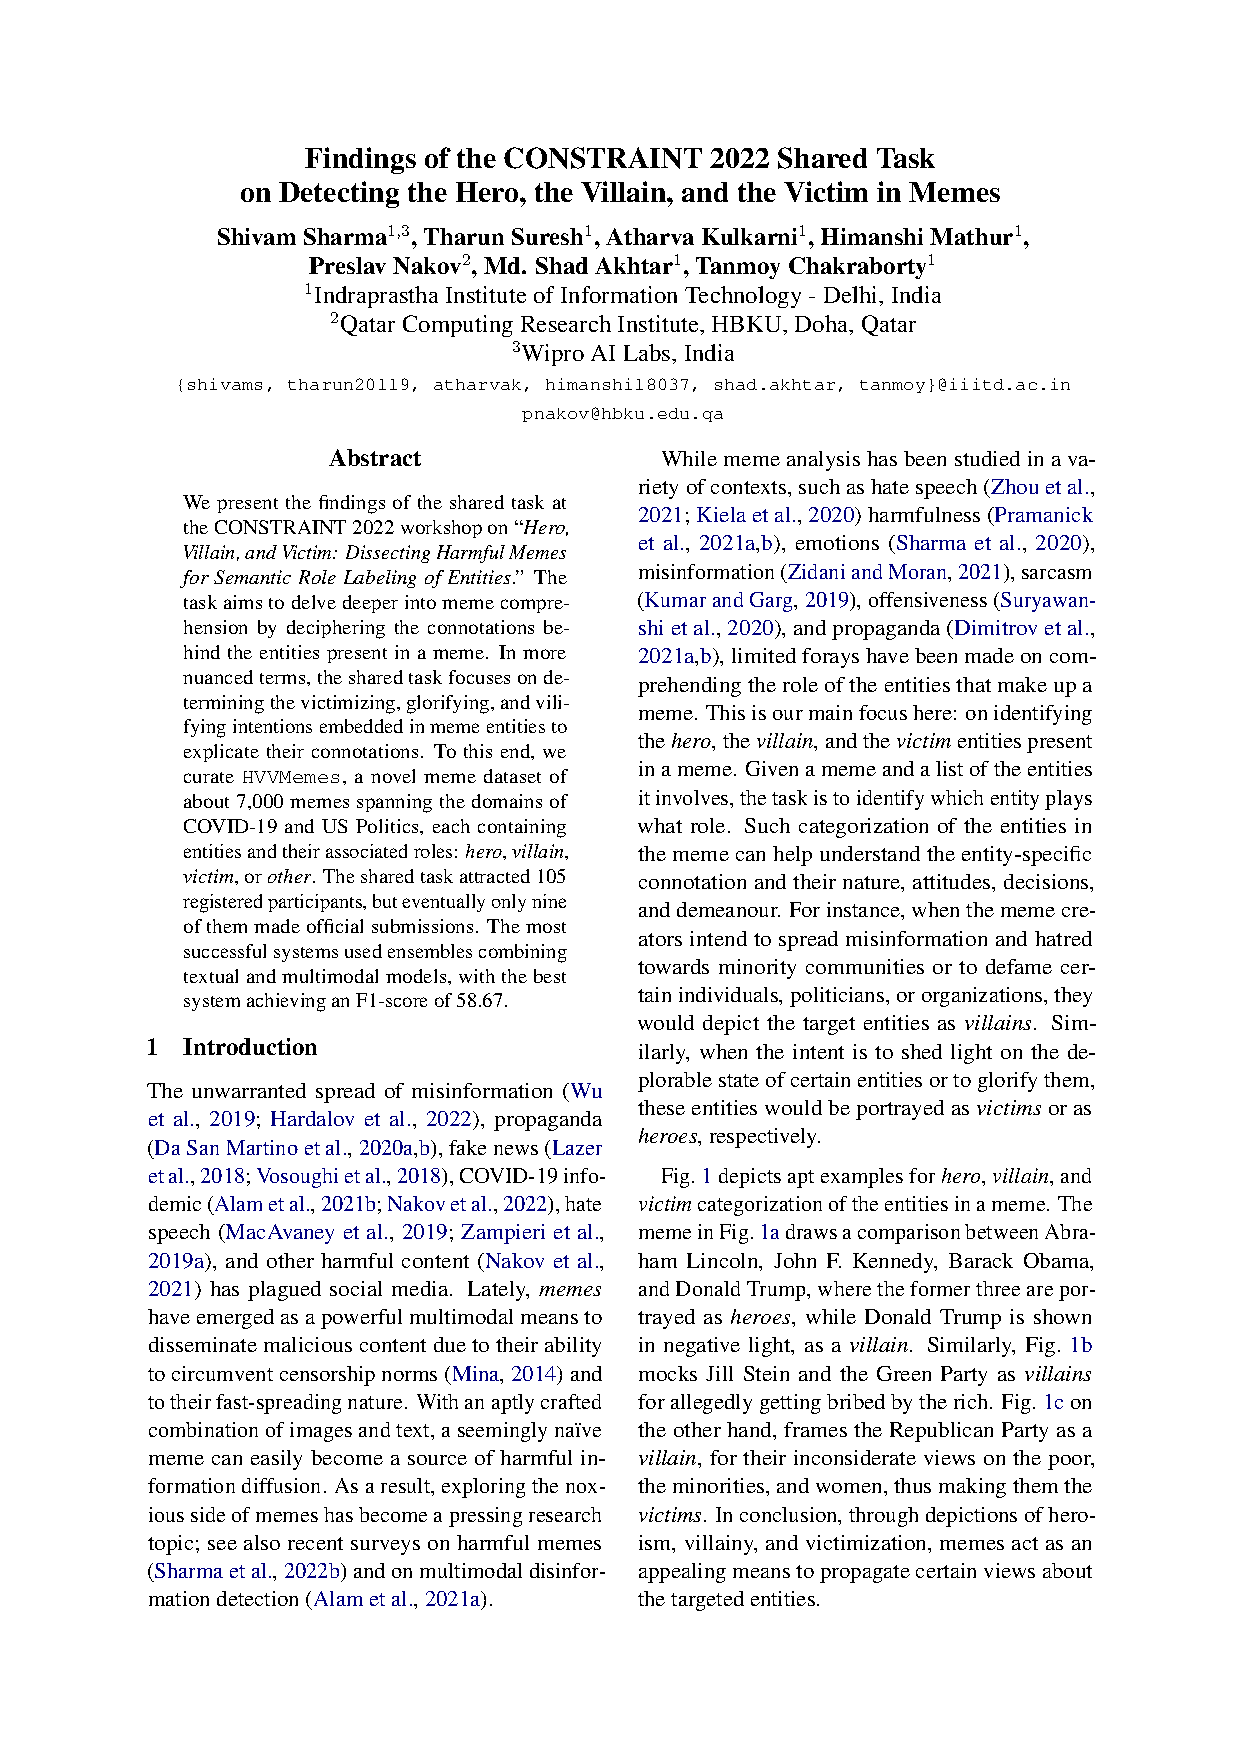
\includepdf[pagecommand={\thispagestyle{plain}},pages=-]{./papers/10.pdf}
  \addcontentsline{toc}{section}{TEMPLATE_TITLE}
  \AddToShipoutPicture*{
    \setlength{\unitlength}{1mm}
    \footnotesize

            
    \put(0,14){\parbox[t]{\paperwidth}{\centering
    							\emph{Proceedings of the Workshop on Combating Online Hostile Posts in Regional Languages during Emergency Situations}, pages 12 - 18 \\
  	  						May 27, 2022 \textcopyright
  							2022 Association for Computational Linguistics}}
  }
  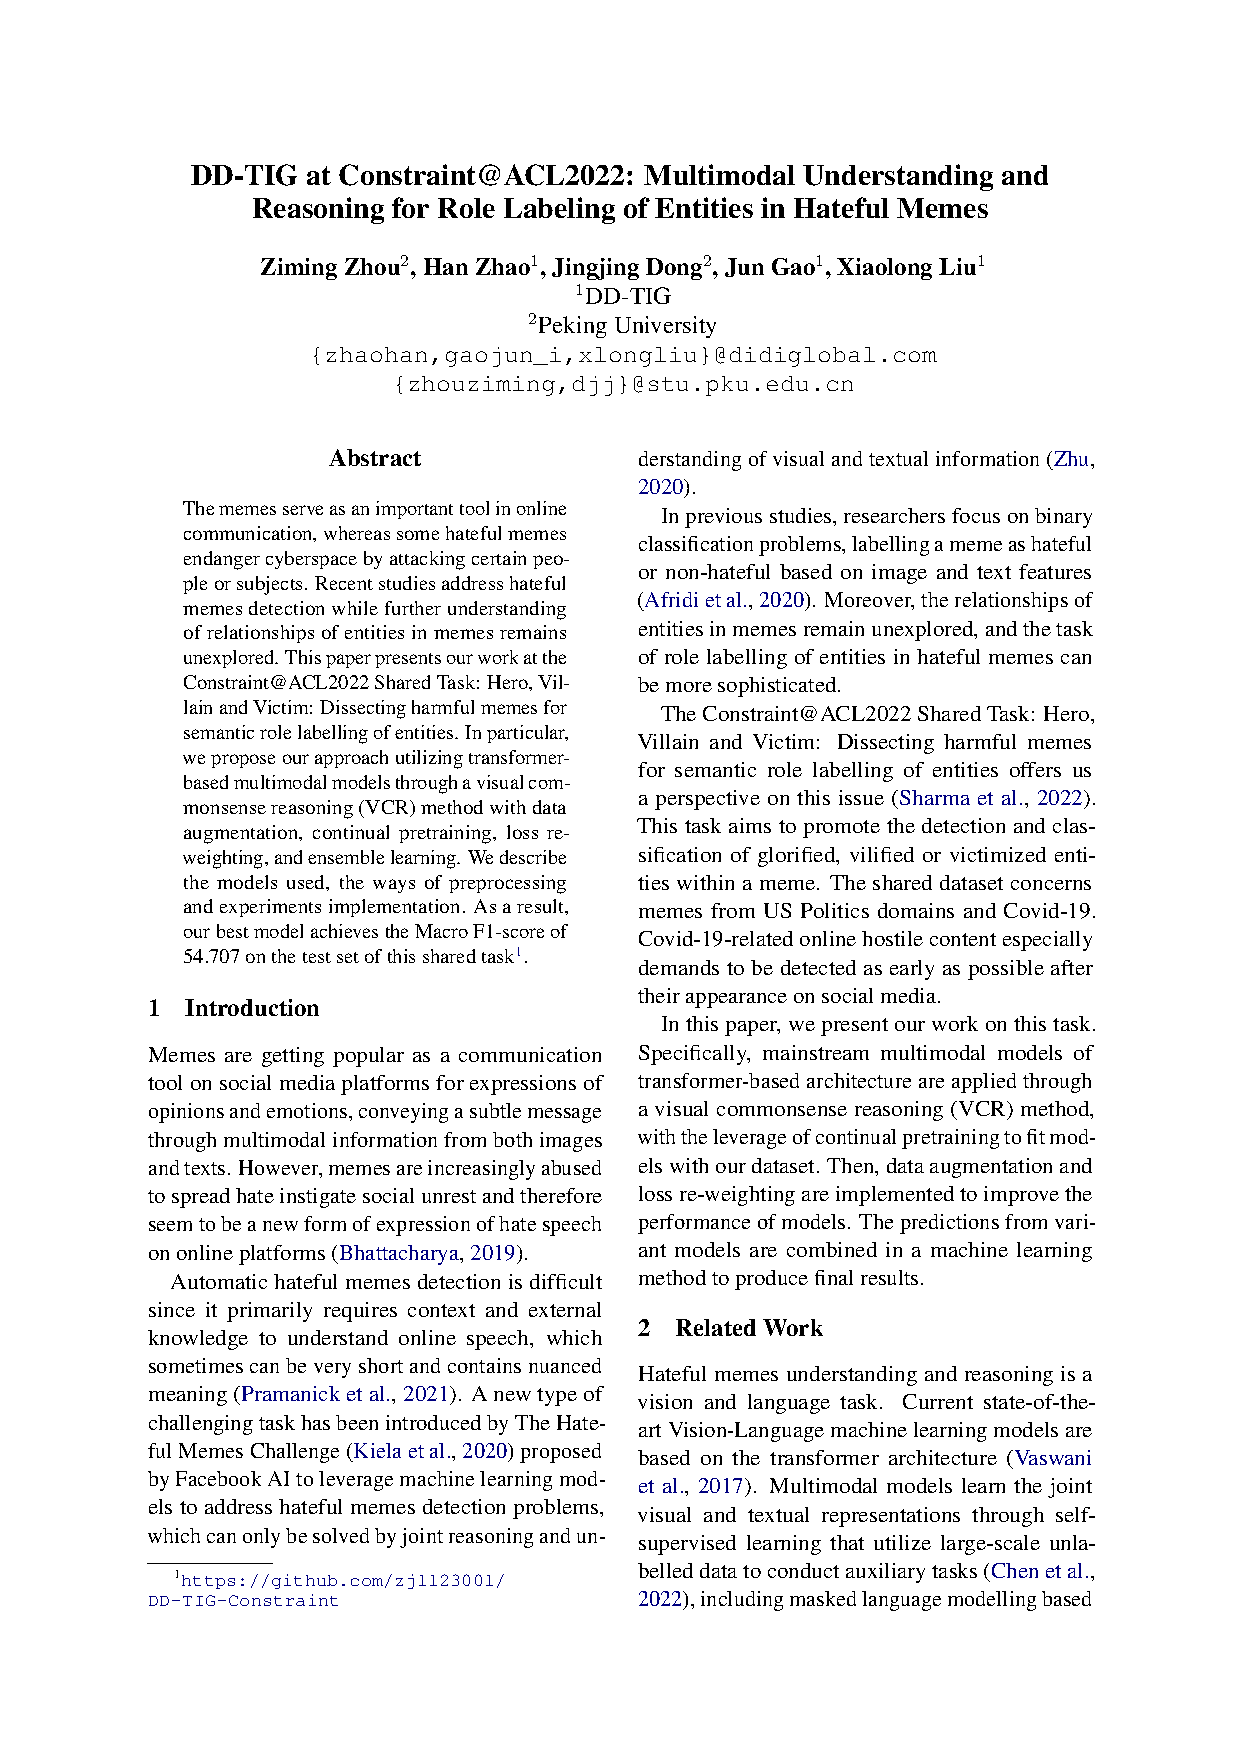
\includepdf[pagecommand={\thispagestyle{plain}},pages=-]{./papers/4.pdf}
  \addcontentsline{toc}{section}{TEMPLATE_TITLE}
  \AddToShipoutPicture*{
    \setlength{\unitlength}{1mm}
    \footnotesize

            
    \put(0,14){\parbox[t]{\paperwidth}{\centering
    							\emph{Proceedings of the Workshop on Combating Online Hostile Posts in Regional Languages during Emergency Situations}, pages 19 - 23 \\
  	  						May 27, 2022 \textcopyright
  							2022 Association for Computational Linguistics}}
  }
  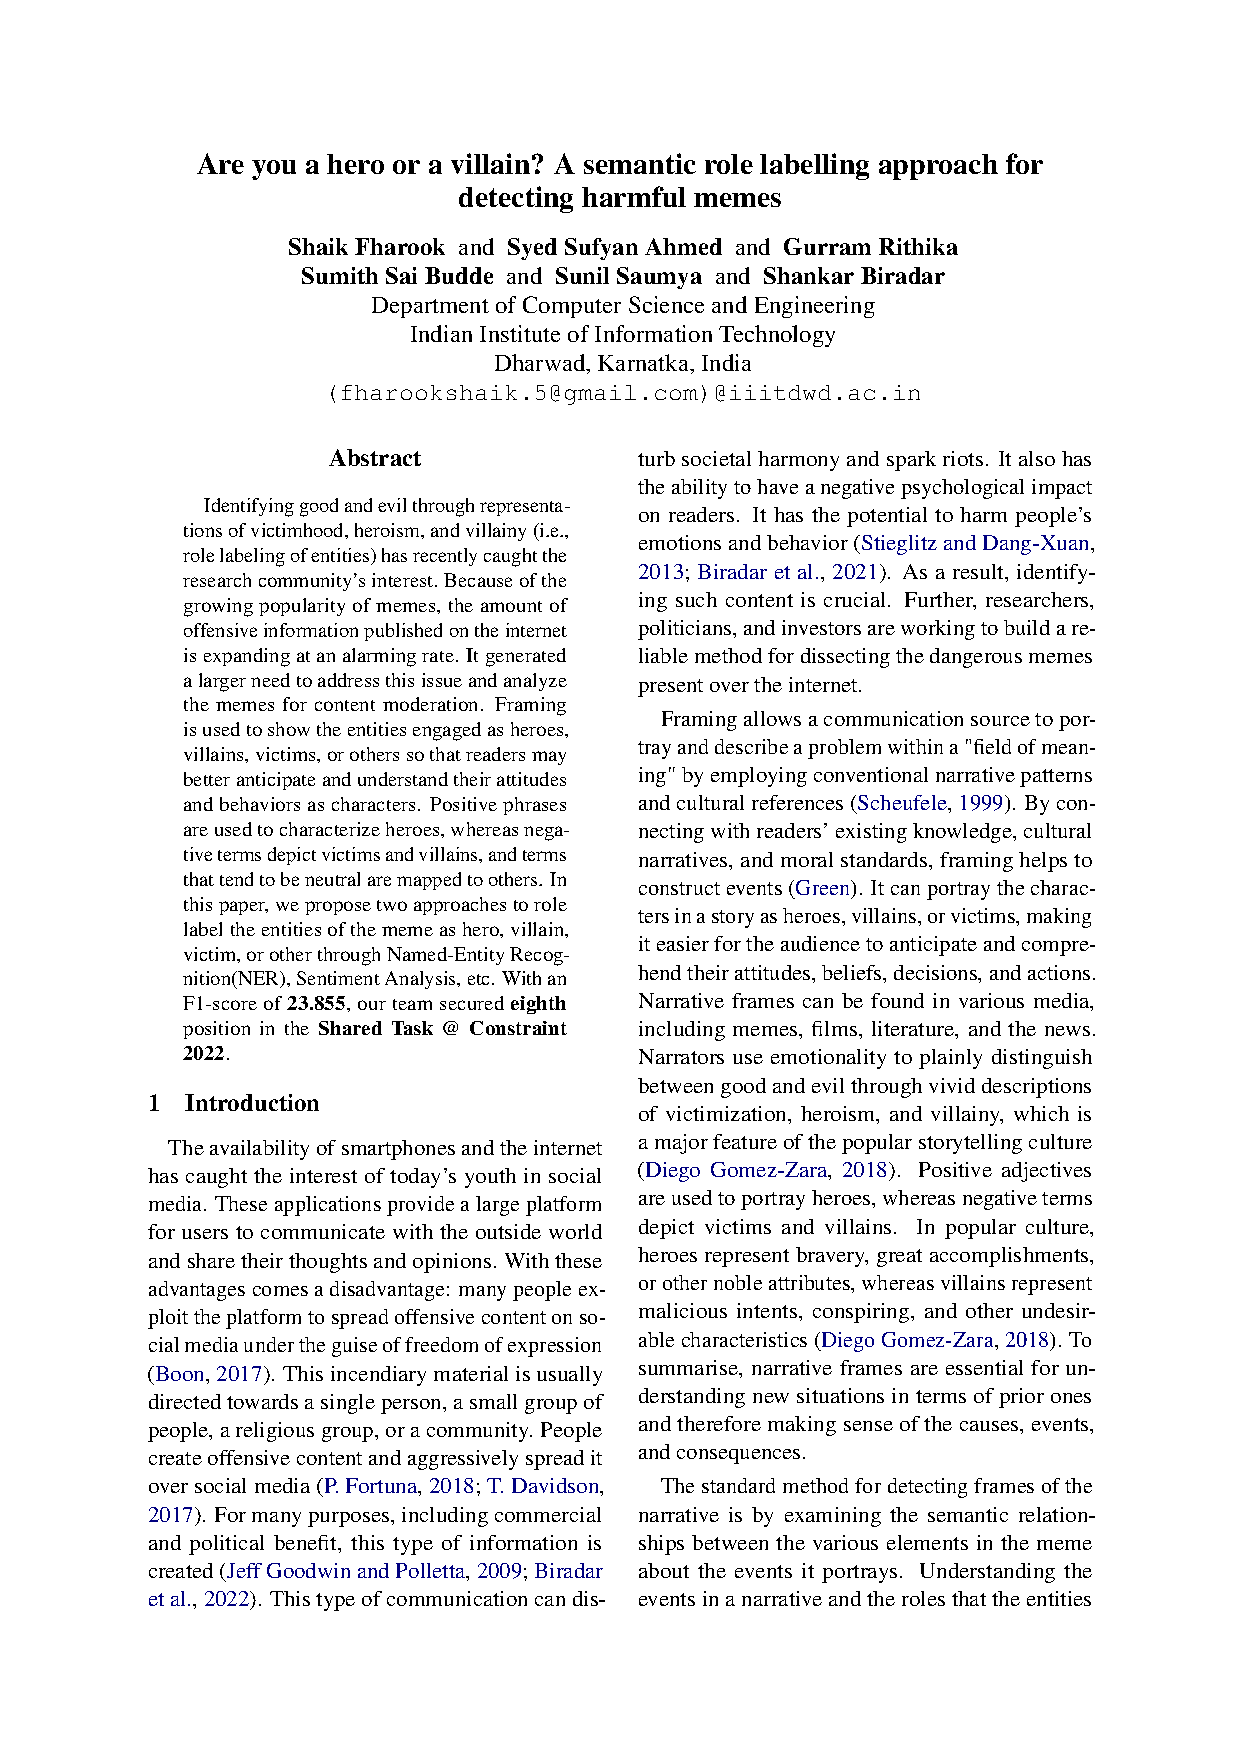
\includepdf[pagecommand={\thispagestyle{plain}},pages=-]{./papers/5.pdf}
  \addcontentsline{toc}{section}{TEMPLATE_TITLE}
  \AddToShipoutPicture*{
    \setlength{\unitlength}{1mm}
    \footnotesize

            
    \put(0,14){\parbox[t]{\paperwidth}{\centering
    							\emph{Proceedings of the Workshop on Combating Online Hostile Posts in Regional Languages during Emergency Situations}, pages 24 - 34 \\
  	  						May 27, 2022 \textcopyright
  							2022 Association for Computational Linguistics}}
  }
  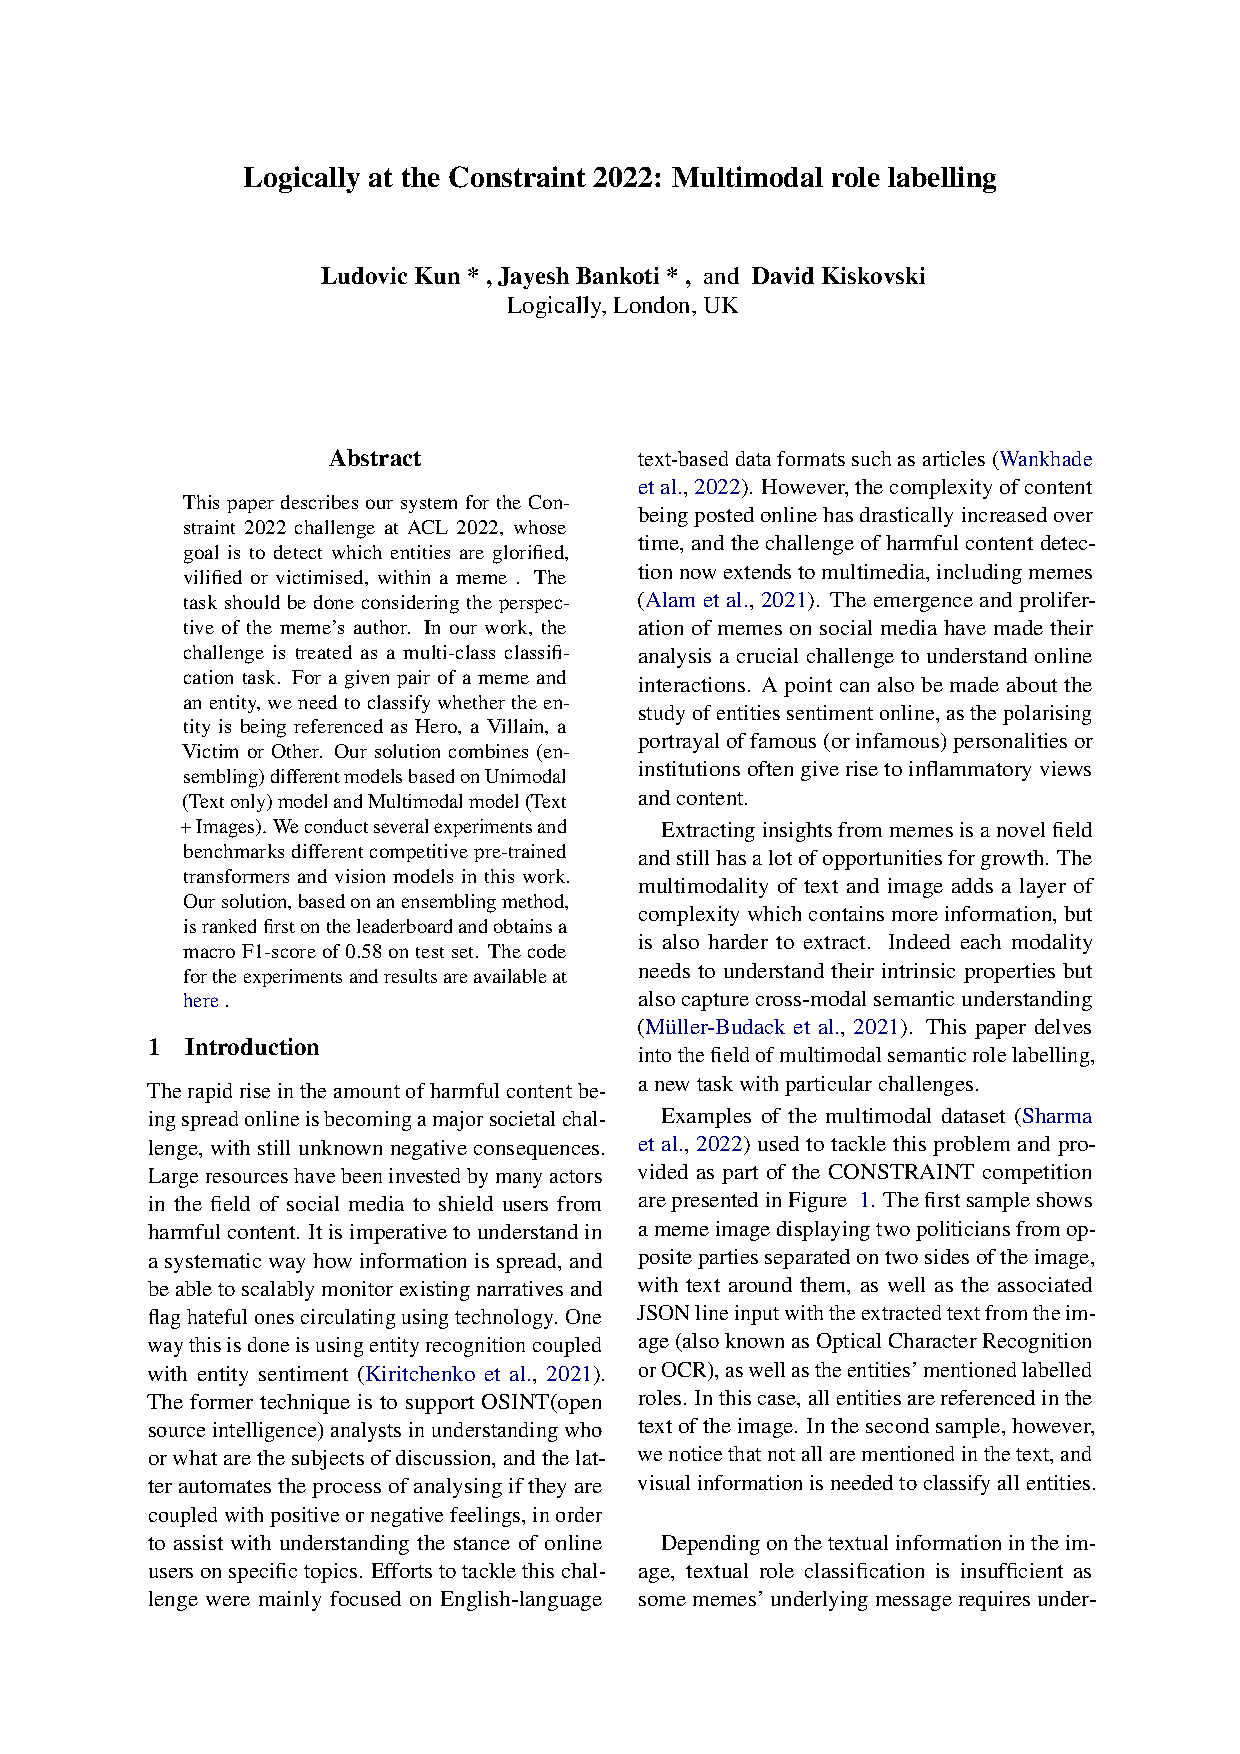
\includepdf[pagecommand={\thispagestyle{plain}},pages=-]{./papers/6.pdf}
  \addcontentsline{toc}{section}{TEMPLATE_TITLE}
  \AddToShipoutPicture*{
    \setlength{\unitlength}{1mm}
    \footnotesize

            
    \put(0,14){\parbox[t]{\paperwidth}{\centering
    							\emph{Proceedings of the Workshop on Combating Online Hostile Posts in Regional Languages during Emergency Situations}, pages 35 - 42 \\
  	  						May 27, 2022 \textcopyright
  							2022 Association for Computational Linguistics}}
  }
  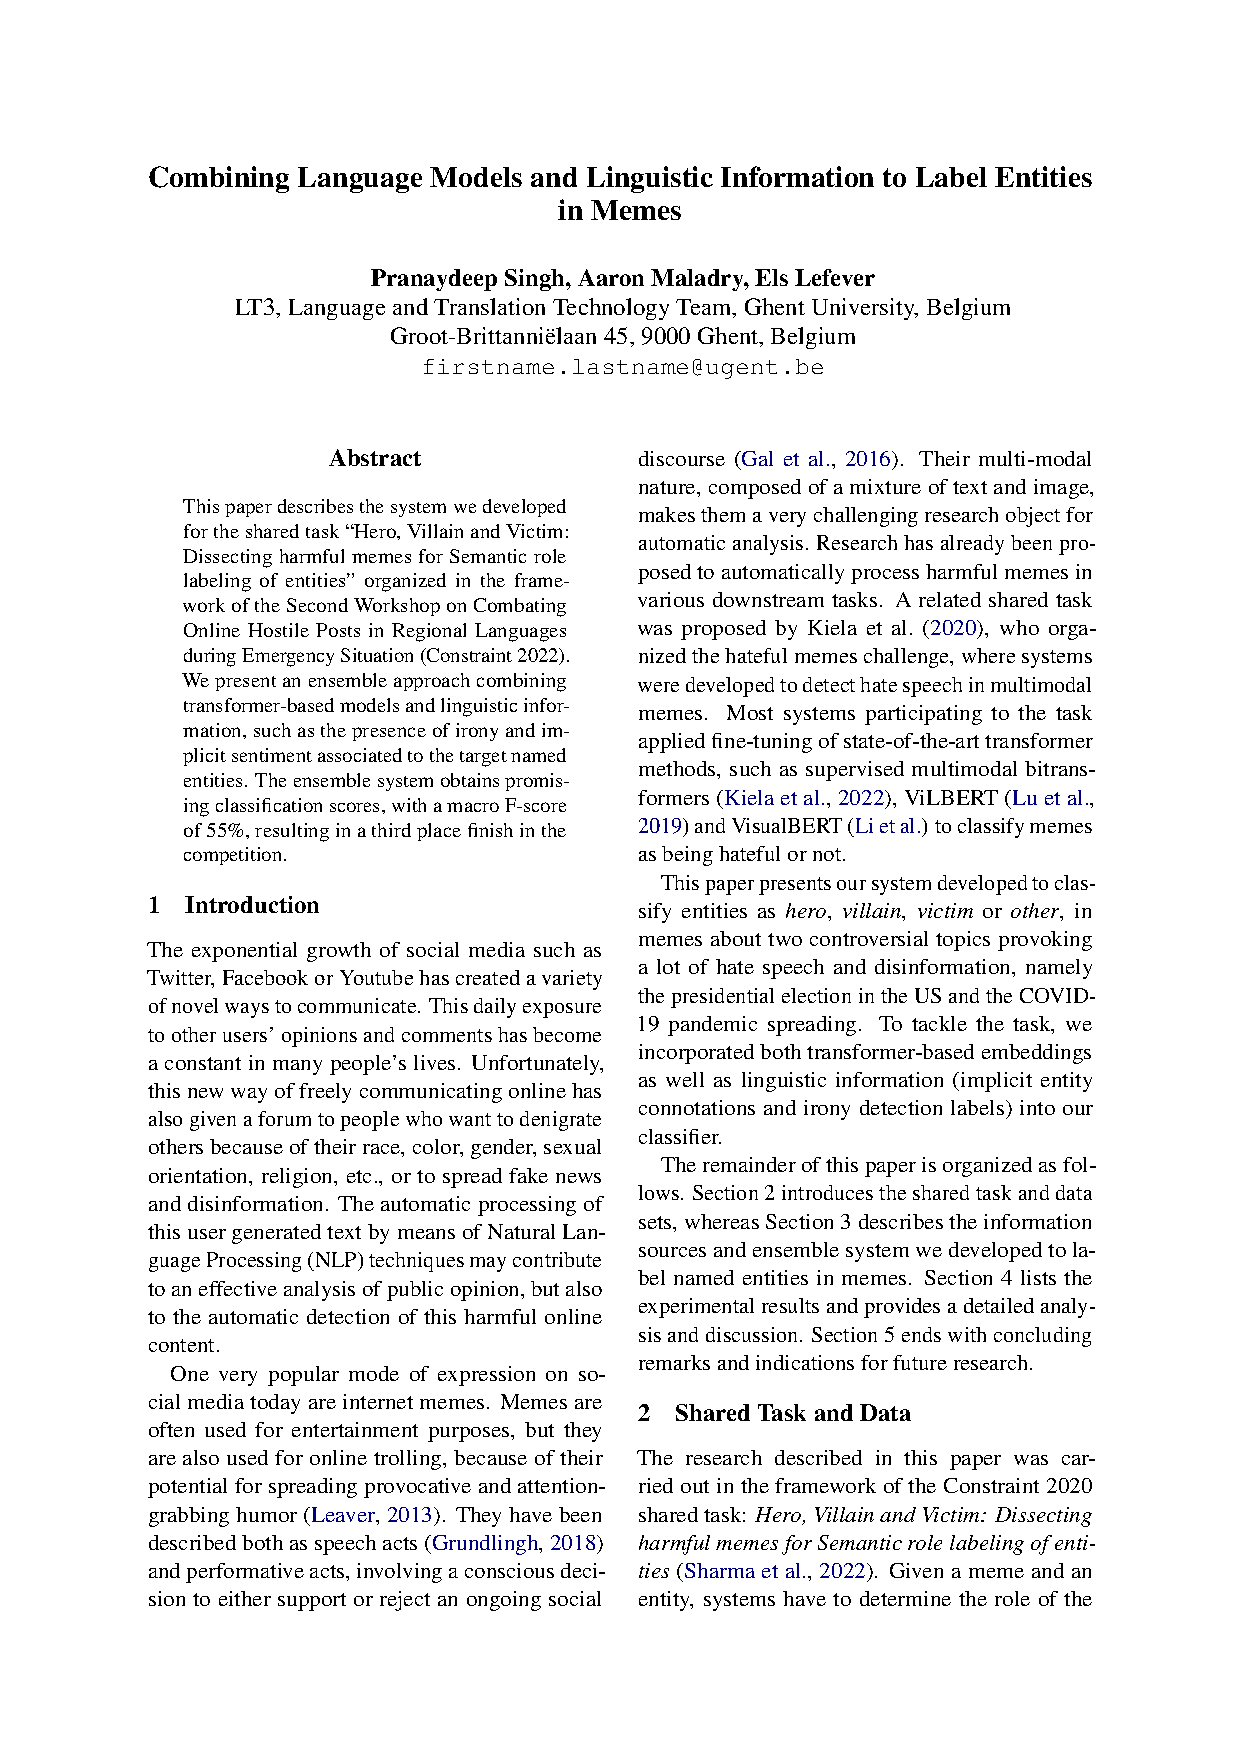
\includepdf[pagecommand={\thispagestyle{plain}},pages=-]{./papers/7.pdf}
  \addcontentsline{toc}{section}{TEMPLATE_TITLE}
  \AddToShipoutPicture*{
    \setlength{\unitlength}{1mm}
    \footnotesize

            
    \put(0,14){\parbox[t]{\paperwidth}{\centering
    							\emph{Proceedings of the Workshop on Combating Online Hostile Posts in Regional Languages during Emergency Situations}, pages 43 - 54 \\
  	  						May 27, 2022 \textcopyright
  							2022 Association for Computational Linguistics}}
  }
  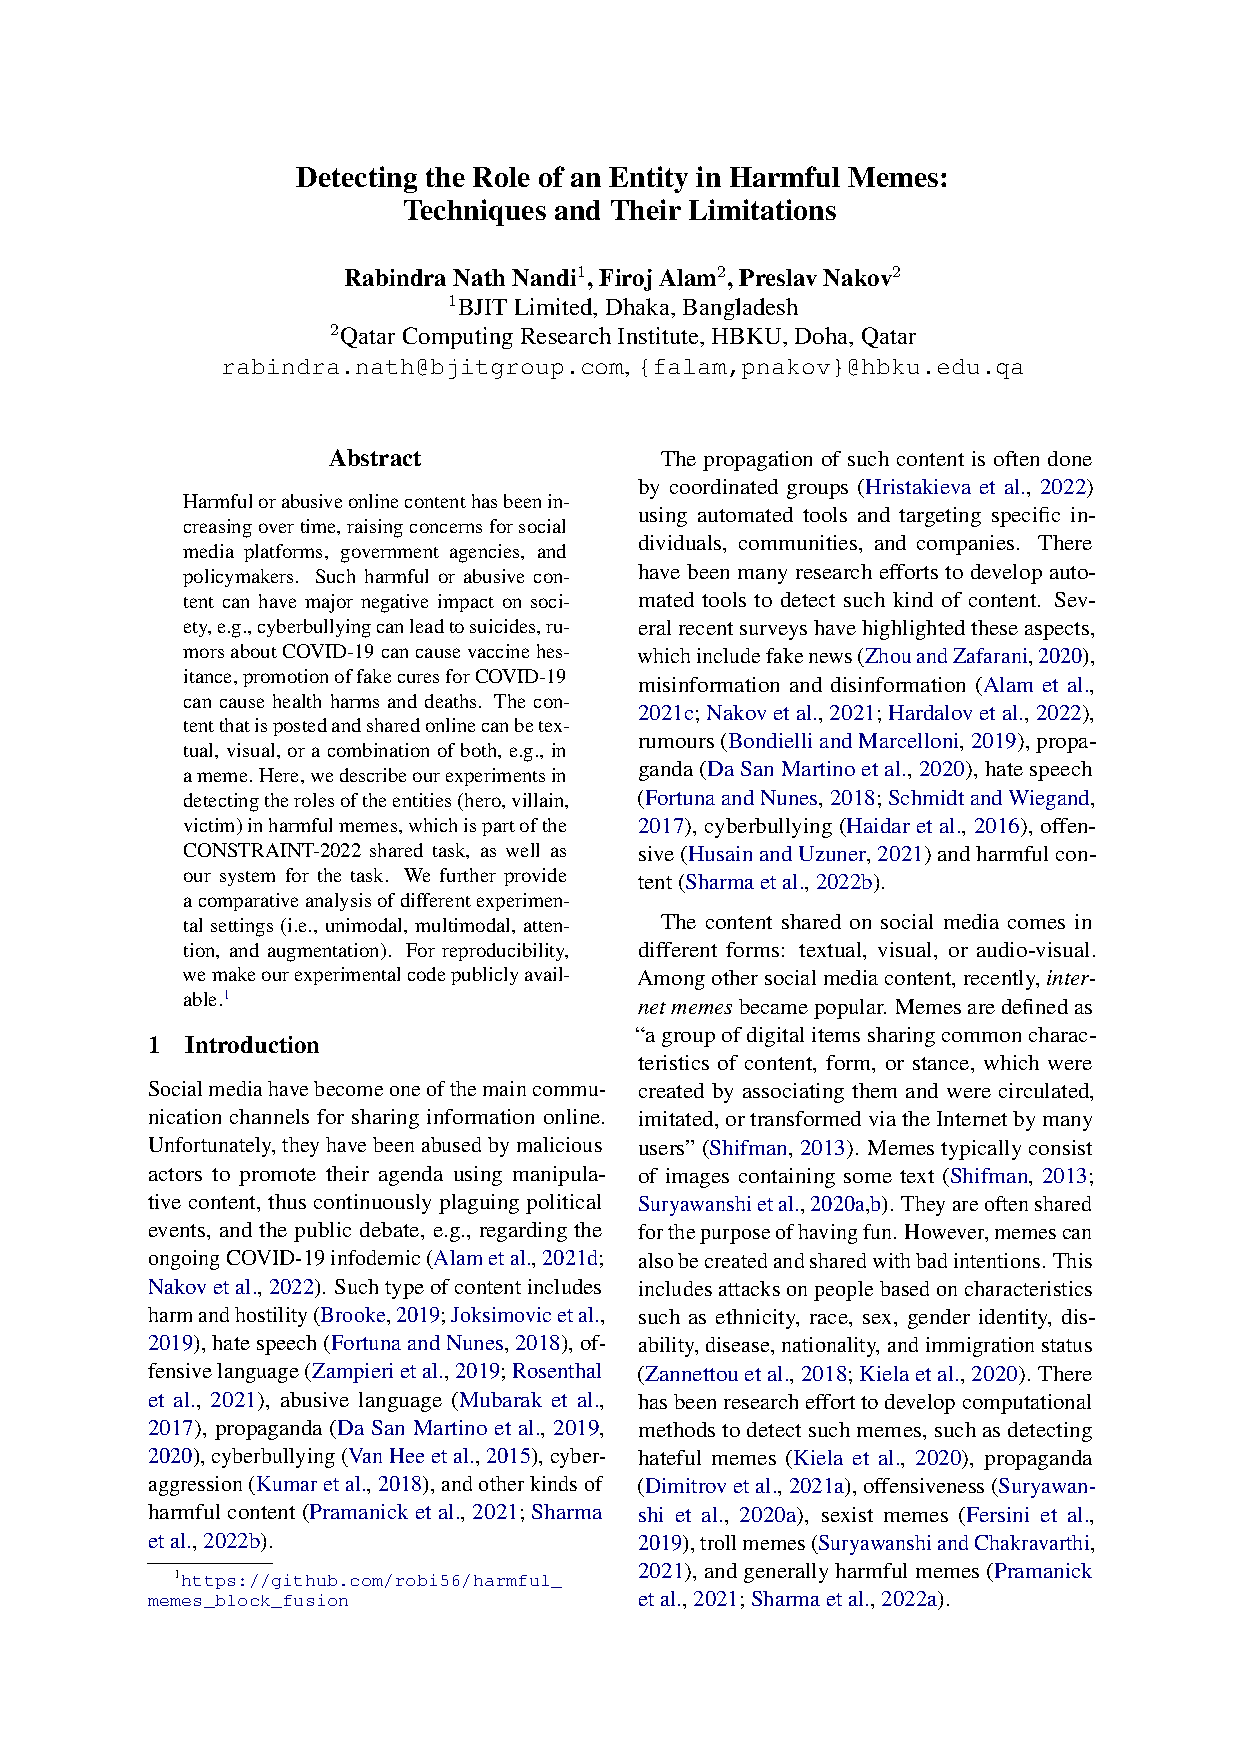
\includepdf[pagecommand={\thispagestyle{plain}},pages=-]{./papers/8.pdf}
  \addcontentsline{toc}{section}{TEMPLATE_TITLE}
  \AddToShipoutPicture*{
    \setlength{\unitlength}{1mm}
    \footnotesize

            
    \put(0,14){\parbox[t]{\paperwidth}{\centering
    							\emph{Proceedings of the Workshop on Combating Online Hostile Posts in Regional Languages during Emergency Situations}, pages 55 - 65 \\
  	  						May 27, 2022 \textcopyright
  							2022 Association for Computational Linguistics}}
  }
  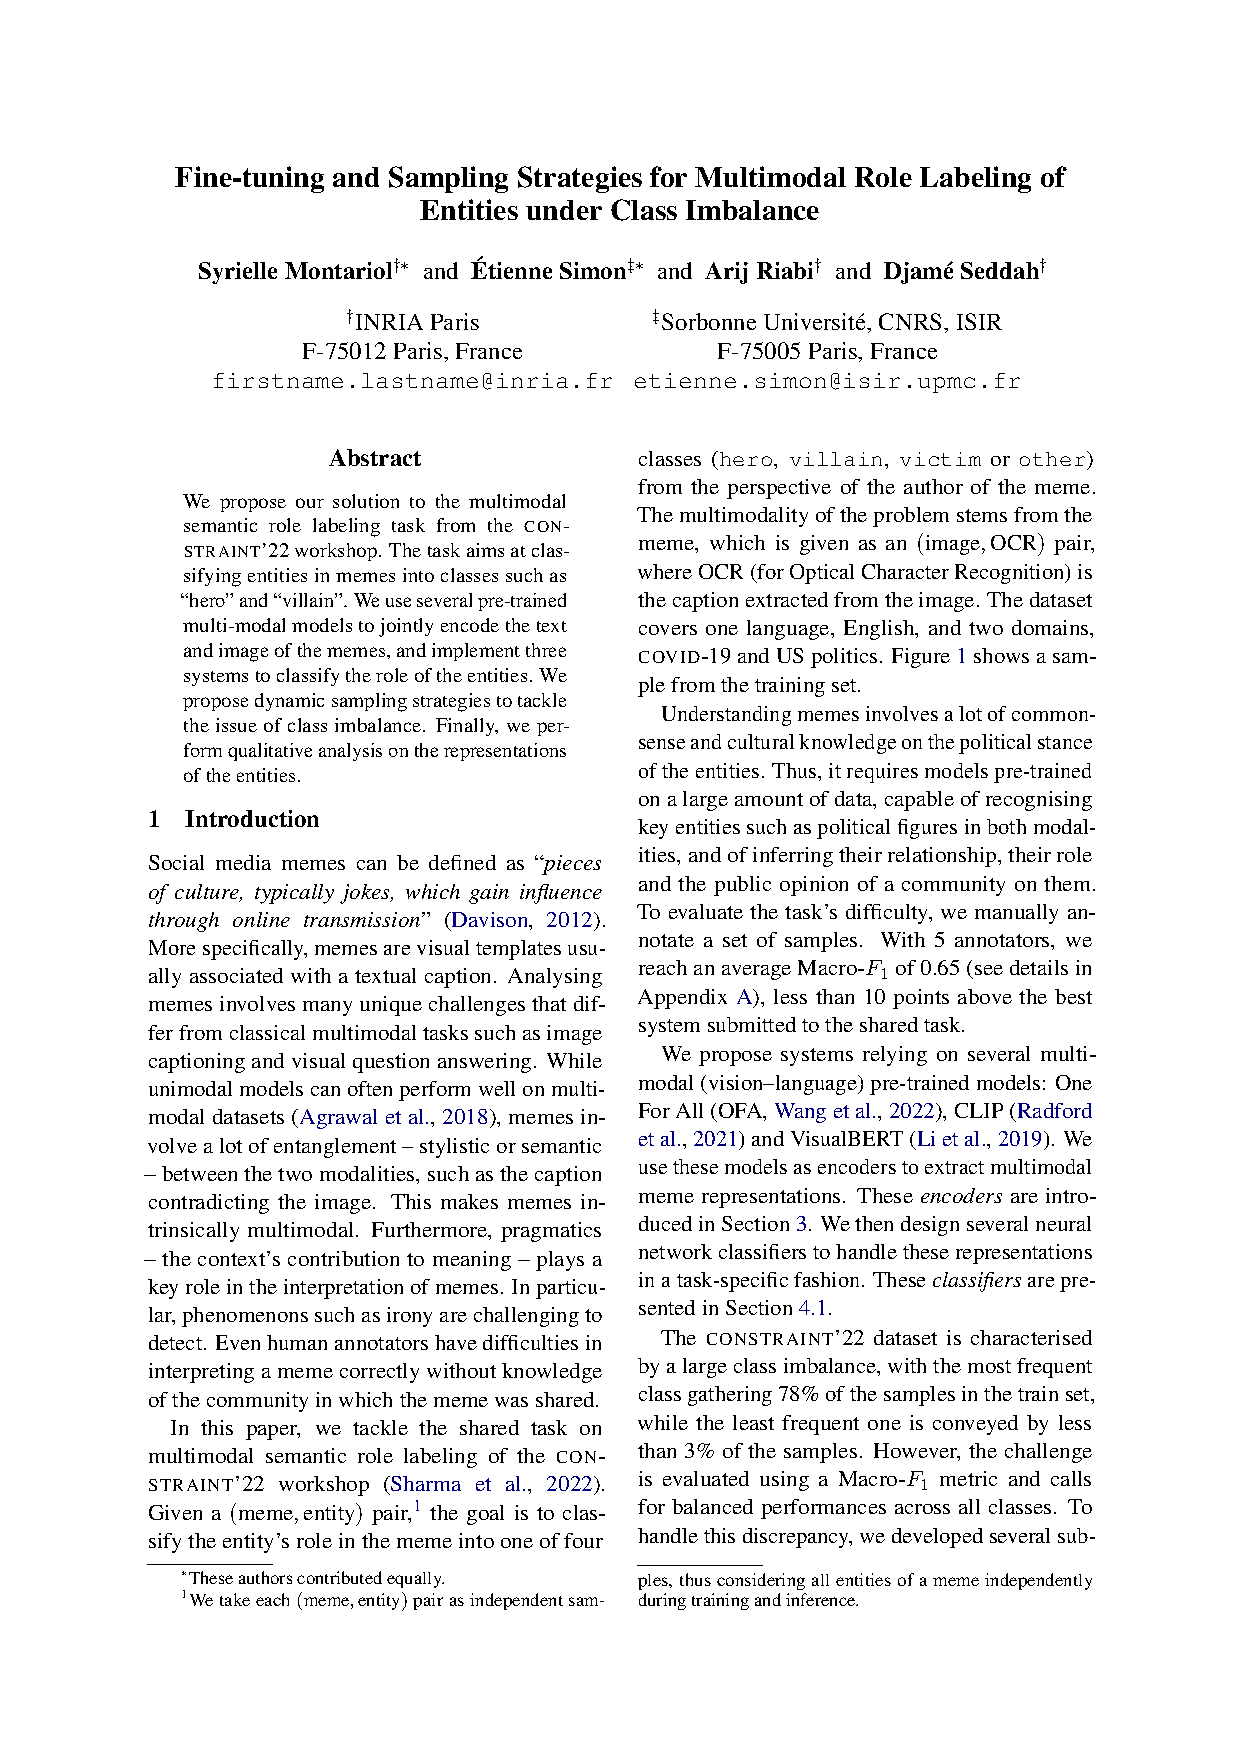
\includepdf[pagecommand={\thispagestyle{plain}},pages=-]{./papers/9.pdf}
  \addcontentsline{toc}{section}{TEMPLATE_TITLE}
  \AddToShipoutPicture*{
    \setlength{\unitlength}{1mm}
    \footnotesize

            
    \put(0,14){\parbox[t]{\paperwidth}{\centering
    							\emph{Proceedings of the Workshop on Combating Online Hostile Posts in Regional Languages during Emergency Situations}, pages 66 - 74 \\
  	  						May 27, 2022 \textcopyright
  							2022 Association for Computational Linguistics}}
  }
  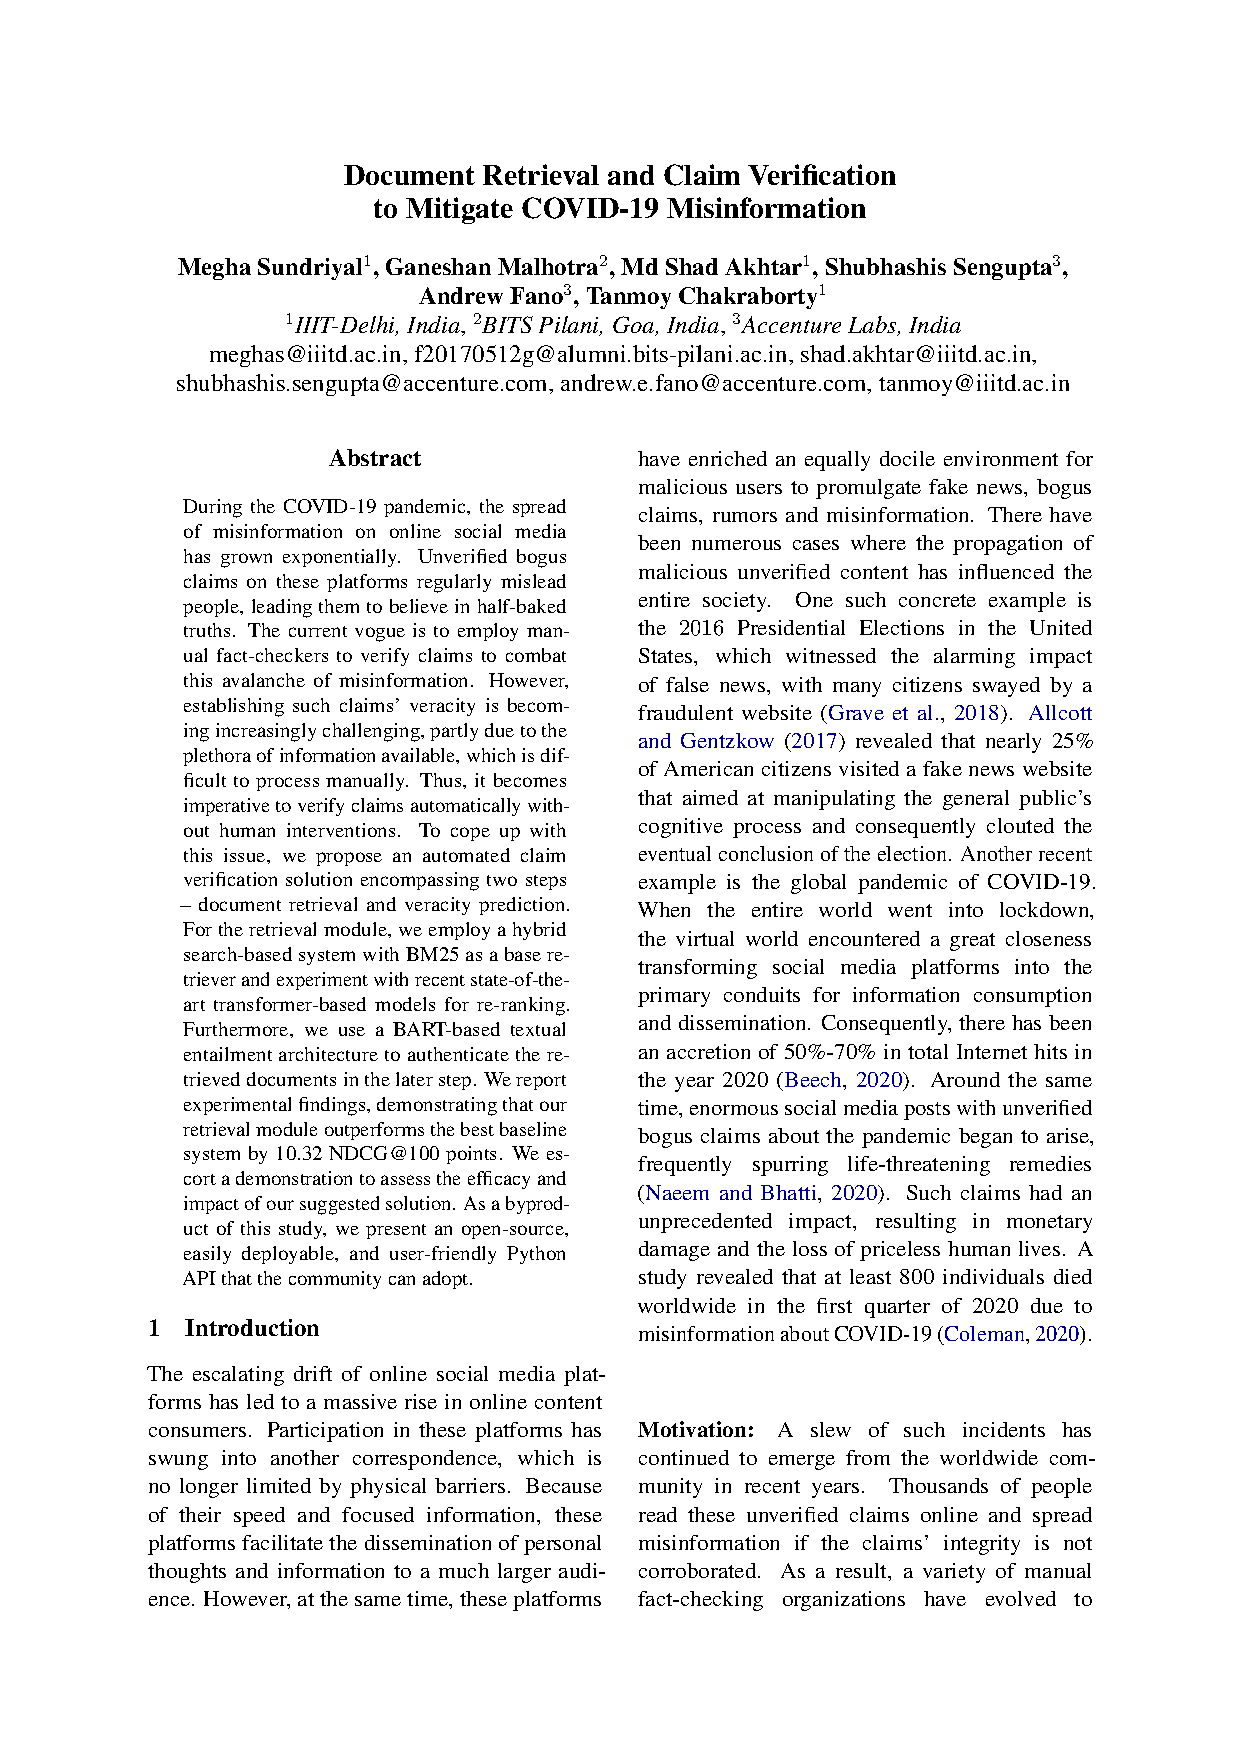
\includepdf[pagecommand={\thispagestyle{plain}},pages=-]{./papers/11.pdf}
  \addcontentsline{toc}{section}{TEMPLATE_TITLE}
  \AddToShipoutPicture*{
    \setlength{\unitlength}{1mm}
    \footnotesize

            
    \put(0,14){\parbox[t]{\paperwidth}{\centering
    							\emph{Proceedings of the Workshop on Combating Online Hostile Posts in Regional Languages during Emergency Situations}, pages 75 - 85 \\
  	  						May 27, 2022 \textcopyright
  							2022 Association for Computational Linguistics}}
  }
  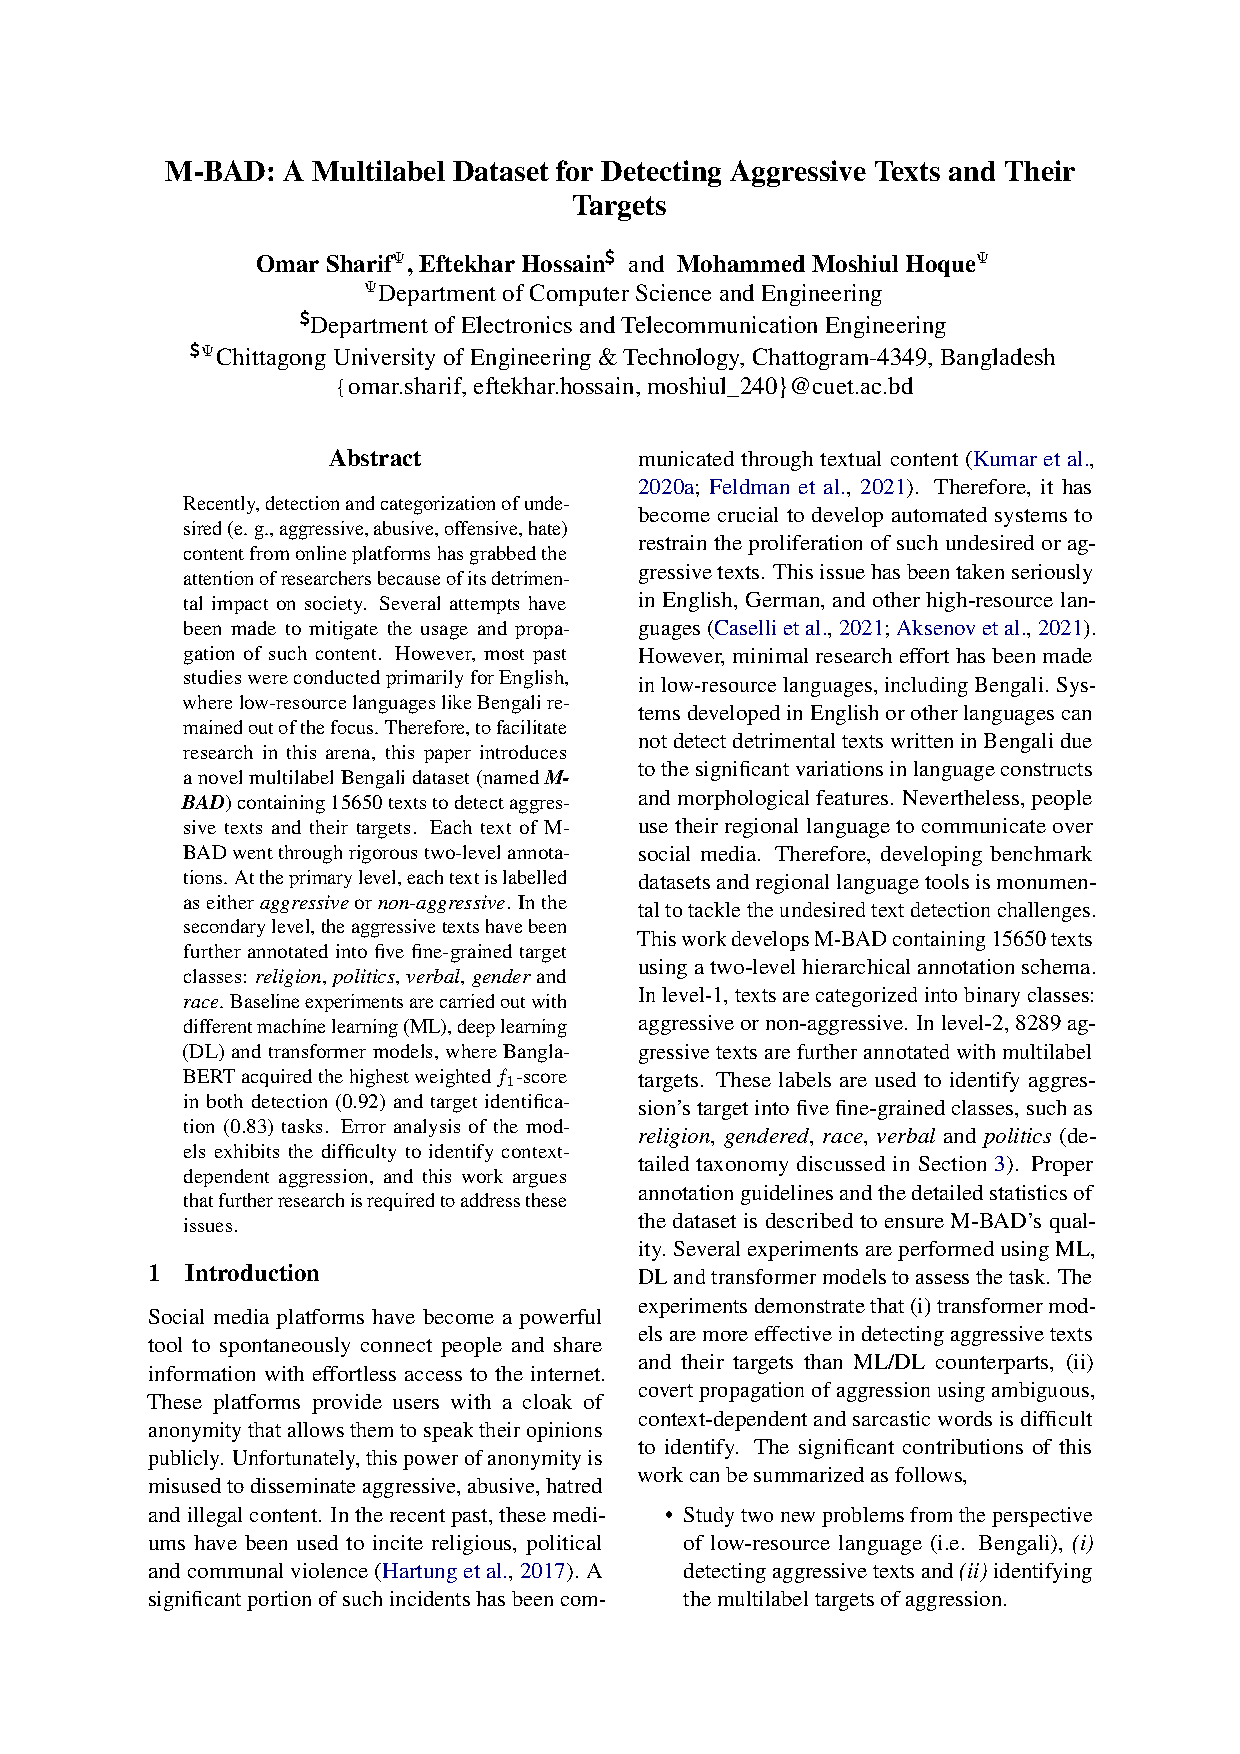
\includepdf[pagecommand={\thispagestyle{plain}},pages=-]{./papers/1.pdf}
  \addcontentsline{toc}{section}{TEMPLATE_TITLE}
  \AddToShipoutPicture*{
    \setlength{\unitlength}{1mm}
    \footnotesize

            
    \put(0,14){\parbox[t]{\paperwidth}{\centering
    							\emph{Proceedings of the Workshop on Combating Online Hostile Posts in Regional Languages during Emergency Situations}, pages 86 - 94 \\
  	  						May 27, 2022 \textcopyright
  							2022 Association for Computational Linguistics}}
  }
  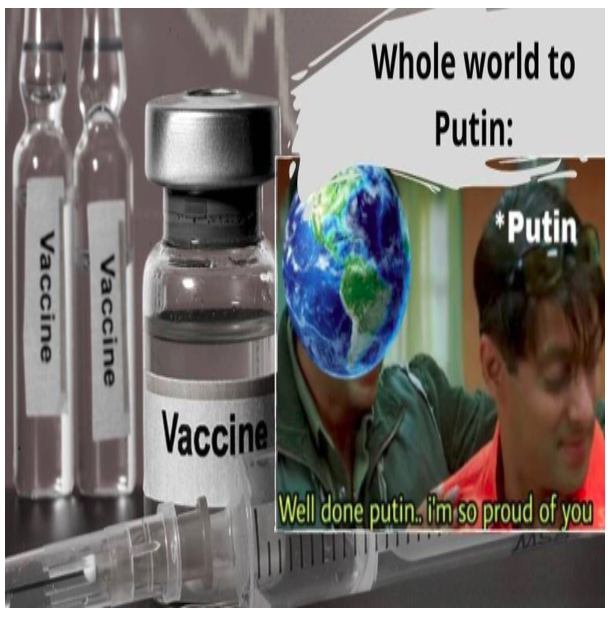
\includepdf[pagecommand={\thispagestyle{plain}},pages=-]{./papers/2.pdf}
  \addcontentsline{toc}{section}{TEMPLATE_TITLE}
  \AddToShipoutPicture*{
    \setlength{\unitlength}{1mm}
    \footnotesize

            
    \put(0,14){\parbox[t]{\paperwidth}{\centering
    							\emph{Proceedings of the Workshop on Combating Online Hostile Posts in Regional Languages during Emergency Situations}, pages 95 - 102 \\
  	  						May 27, 2022 \textcopyright
  							2022 Association for Computational Linguistics}}
  }
  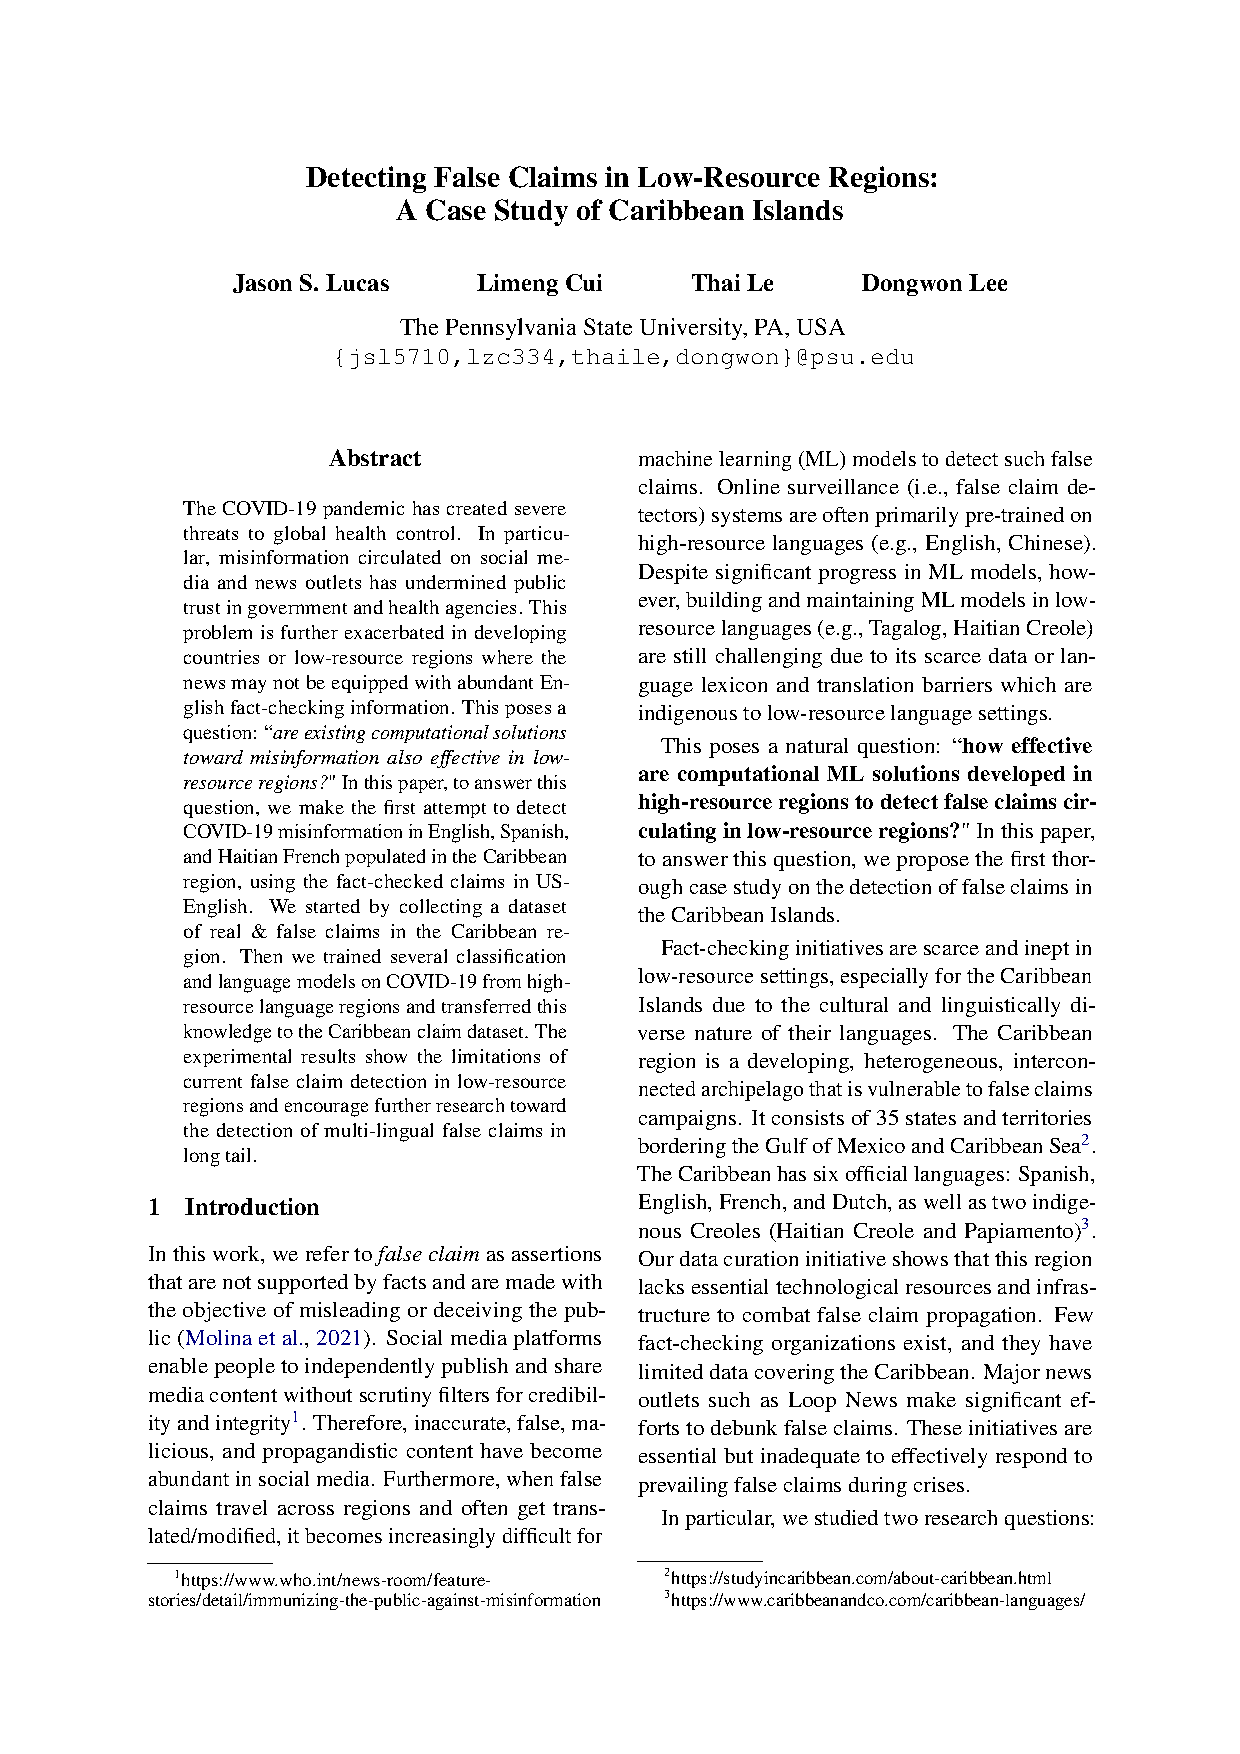
\includepdf[pagecommand={\thispagestyle{plain}},pages=-]{./papers/3.pdf}

%%%%%%%%%%%%%%%%
% Author Index %
%%%%%%%%%%%%%%%%
\begin{huge}
Author Index
\end{huge}
\vspace*{1em}
\begin{multicols}{2}
Akhtar, Md Shad, \hyperlink{page.66}{66}\\
Akhtar, Md. Shad, \hyperlink{page.1}{1}\\
Alam, Firoj, \hyperlink{page.43}{43}\\
\\ % Extra space between new letters.
Bankoti, Jayesh, \hyperlink{page.24}{24}\\
Biradar, Shankar, \hyperlink{page.19}{19}\\
Budde, Sumith Sai, \hyperlink{page.19}{19}\\
\\ % Extra space between new letters.
Chakraborty, Tanmoy, \hyperlink{page.1}{1}, \hyperlink{page.66}{66}\\
Choi, Hyewon, \hyperlink{page.86}{86}\\
Cui, Limeng, \hyperlink{page.95}{95}\\
\\ % Extra space between new letters.
Dong, Jingjing, \hyperlink{page.12}{12}\\
\\ % Extra space between new letters.
Fano, Andrew, \hyperlink{page.66}{66}\\
Fharook, Shaik, \hyperlink{page.19}{19}\\
\\ % Extra space between new letters.
Gao, Jun, \hyperlink{page.12}{12}\\
\\ % Extra space between new letters.
Hoque, Mohammed Moshiul, \hyperlink{page.75}{75}\\
Hossain, Eftekhar, \hyperlink{page.75}{75}\\
\\ % Extra space between new letters.
Kiskovski, David, \hyperlink{page.24}{24}\\
Kulkarni, Atharva, \hyperlink{page.1}{1}\\
Kun, Ludovic, \hyperlink{page.24}{24}\\
\\ % Extra space between new letters.
Le, Thai, \hyperlink{page.95}{95}\\
Lee, Dongwon, \hyperlink{page.95}{95}\\
Lefever, Els, \hyperlink{page.35}{35}\\
Liu, Xiaolong, \hyperlink{page.12}{12}\\
Lucas, Jason, \hyperlink{page.95}{95}\\
\\ % Extra space between new letters.
Maladry, Aaron, \hyperlink{page.35}{35}\\
Malhotra, Ganeshan, \hyperlink{page.66}{66}\\
Mathur, Himanshi, \hyperlink{page.1}{1}\\
Montariol, Syrielle, \hyperlink{page.55}{55}\\
\\ % Extra space between new letters.
Nakov, Preslav, \hyperlink{page.1}{1}, \hyperlink{page.43}{43}\\
Nandi, Rabindra Nath, \hyperlink{page.43}{43}\\
\\ % Extra space between new letters.
Park, Kunwoo, \hyperlink{page.86}{86}\\
\\ % Extra space between new letters.
Riabi, Arij, \hyperlink{page.55}{55}\\
Rithika, Gurram, \hyperlink{page.19}{19}\\
\\ % Extra space between new letters.
Saumya, Sunil, \hyperlink{page.19}{19}\\
Seddah, Djamé, \hyperlink{page.55}{55}\\
Sengupta, Shubhashis, \hyperlink{page.66}{66}\\
Sharif, Omar, \hyperlink{page.75}{75}\\
Sharma, Shivam, \hyperlink{page.1}{1}\\
Simon, Étienne, \hyperlink{page.55}{55}\\
Singh, Pranaydeep, \hyperlink{page.35}{35}\\
Sufyan Ahmed, Syed, \hyperlink{page.19}{19}\\
Sundriyal, Megha, \hyperlink{page.66}{66}\\
Suresh, Tharun, \hyperlink{page.1}{1}\\
\\ % Extra space between new letters.
Yoon, Seunghyun, \hyperlink{page.86}{86}\\
Yoon, Yejun, \hyperlink{page.86}{86}\\
\\ % Extra space between new letters.
Zhao, Han, \hyperlink{page.12}{12}\\
Zhou, Ziming, \hyperlink{page.12}{12}\\
\\ % Extra space between new letters.
\end{multicols}


\end{document}